
\section{Lot-sizing with hierarchical types}

In this section, we consider a related problem where facilities and clients are embedded in time, and thus may correspond to orders and demands occurring over time. Let order $i$ occur at time $\tau(i)$ and demand $j$ occur at time $\tau(j)$. We still have the hierarchical type tree as in \textit{facility location with hierarchical types}. For a client $j$ to be served by facility $i$, in addition to the type constraint $t(j) \le t(i)$, we also have the time constraint, $\tau(i) \le \tau(j)$. For the assignment cost $c_{ij}$, we have a non-decreasing property: for two facilities $i,i'$ and client $j$ with $\tau(i) \le \tau(i') \le \tau(j)$, we have $c_{ij} \ge c_{i'j}$. Also, $c_{ij} = \infty$ if $\tau(i) > \tau(j)$.

\subsection{A dynamic programming algorithm}

We now describe a polynomial-time dynamic programming (DP) formulation to solve
the lot-sizing problem with hierarchical types. For this, we need some new notation. Considering a type tree $\mathcal{T}$, we define $\mathcal{T}(t)$ to be the subtree of $\mathcal{T}$ rooted at $t$ if $t \in \mathcal{T}$, and $\emptyset$ otherwise. We also use $C_\mathcal{T}(t)$ to denote the set of children of $t$ in $\mathcal{T}$. %Also, we use $j(\mathcal{T}(t),i)$ for type $t$ and facility $i$ to denote the client $j$ that has type $t(j) \in \mathcal{T}(t)$ and satisfies $\tau(j)<\tau(i)$, such that $\tau(j)$ is maximized.
%
For convenience we add a dummy facility $\chi$ of the root type occurring at $\tau(\chi) = -\infty$ with opening cost $f_\chi = 0$ such that $c_{\chi j} = \infty$ for any client $j$.

Now, for any facility $i$, any type $t$ satisfying $t \le t(i)$, and any time $\tau > \tau(i)$ we define $\mathcal{L}(i,\mathcal{T}(t), \tau)$ to be the cost of the optimal solution for the subset of the clients and facilities contained in the interval $[\tau(i),\tau)$ that have types contained in the subtree rooted at $t$, i.e., $\mathcal{T}(t)$, with the extra assumption that $i$ has opening cost $f_i = 0$. Thus, the optimal overall cost of the lot-sizing problem is $\mathcal{L}(\chi, \mathcal{T}, \infty)$. Note that there are at most $|\mathcal{D}|$ values for the third element that are of interest, and therefore there are a total of $O(|\mathcal{F}||\mathcal{T}||\mathcal{D}|)$ distinct sub-problems.

The base case of the DP is when the type tree has depth zero, and therefore the optimal
solution has cost $0$. Let us calculate $\mathcal{L}$ using a recursive formula that uses
induction on the depth of the type tree, each time finding the latest facility of the root
type that is opened in the optimal solution. For this, we can establish the following
recurrence. %recursive formula:

\begin{align*}
\mathcal{L}(i, \mathcal{T}(t), \tau) = \min \Big\{
    \sum_{j: t(j)=t, \tau(i) \leq \tau(j) < \tau} c_{ij} + \sum_{t'\in C_\mathcal{T}(t)}  \mathcal{L}(i, \mathcal{T}(t'), \tau),\\
    \min_{i': t(i')=t, \tau(i) < \tau(i') < \tau} \{
        f_{i'}+\mathcal{L}(i, \mathcal{T}(t), \tau(i')) + \sum_{t'\in C_\mathcal{T}(t)} \mathcal{L}(\tau(i'), \mathcal{T}(t'), \tau)
    \}
\Big\}
\end{align*}

The first case of the outer min corresponds to the scenario when no facilities of type $t$ are opened in the optimal solution in the interval $[\tau(i),\tau)$, other than $i$. Here, all clients of type $t$ will be served by $i$, and the rest of the solution can be separately calculated for each of the type trees $T(t')$ for all $t'\in C_\mathcal{T}(t)$, and be summed to get the total cost.

The second case considers the facility $i'$ that is the last facility of type $t$ opened
after $i$ and by time $\tau$. Here, the optimal solution for the interval
$[\tau(i'),\tau)$ is calculated as in the previous case, and the optimal solution for the interval $[\tau(i),\tau(i')]$ is calculated by recursing on $\mathcal{L}(\tau(i'), \mathcal{T}(t'), \tau)$.

Together, the two cases cover all possibilities for the latest facility of type $t$ that is opened in the time interval $[\tau(i), \tau)$ and therefore at some point the optimal solution is considered. Each update can be implemented in $O(|\mathcal{F}|+|\mathcal{D}|)$ given that the facilites and clients of each type are maintained sorted by occurence time, and therefore the total runtime is bounded by $O(|\mathcal{F}|^2|\mathcal{T}||\mathcal{D}|+|\mathcal{F}||\mathcal{T}||\mathcal{D}|^2)$. %This yields the following theorem.

\begin{thm}
There exists a polynomial-time dynamic programming algorithm
to solve the hierarchical lot-sizing problem.
\end{thm}



\subsection{An integrality gap example}

Interestingly, although this problem admits polynomial solution, we can provide an example where the natural linear program has an integrability gap of $\frac{3}{4}$. We need only two types, say $a$ and $b$, where $a$ is the root type and $b$ is the only leaf type.

The instance consists of three facilities $f_1, f_2,$ and $f_3$ and three clients $c_1, c_2,$ and $c_3$ such that $\tau(f_1) < \tau(f_2) < \tau(c_1) < \tau(f_3) < \tau(c_2) < \tau(c_3)$. Also, facilities $f_1$ and $f_3$ and the client $c_3$ are of type $a$ and the rest of clients and facilities are of type $b$. Let us say the opening cost for all facilities is a constant $c$ and the holding costs are $0$, except for $c_{f_1c_2} = \infty$. It is easy to verify that these holding costs are non-decreasing.

\begin{figure}
\centering
\resizebox{9cm}{!}{%
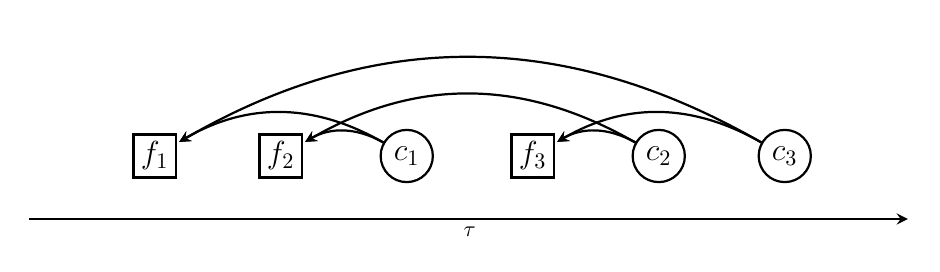
\begin{tikzpicture}[->,>=stealth,shorten >=1pt,auto,node distance=2cm,
                thick,c node/.style={circle,draw,font=\Large\bfseries}, f node/.style={draw,font=\Large\bfseries},scale=0.8, every node/.style={scale=0.8}]


    \draw[->] (-2,-1) to[|->|] node [below] {$\tau$} (12,-1);
    \node[f node] (f1) {$f_1$};
    \node[f node] (f2) [right of=f1] {$f_2$};
    \node[c node] (c1) [right of=f2] {$c_1$};
    \node[f node] (f3) [right of=c1] {$f_3$};
    \node[c node] (c2) [right of=f3] {$c_2$};
    \node[c node] (c3) [right of=c2] {$c_3$};

    \path
    (c1) edge [bend right] (f1);
    \path
    (c1) edge [bend right] (f2);
    \path
    (c2) edge [bend right] (f2);
    \path
    (c2) edge [bend right] (f3);
    \path
    (c3) edge [bend right] (f1);
    \path
    (c3) edge [bend right] (f3);


\end{tikzpicture}
}

\caption{The instance of the lot-sizing problem inducing integrality gap of $4/3$ for LP and the corresponding support of $x$. All drawn arcs correspond to half integral values.}
\label{fig:IGlotsizing}
\end{figure}

Any solution that opens two of the facilities will have a total cost of $2c$ and would be optimal. However, in a fractional solution one can open each facility halfway since each client can be served by two facilities without paying a holding cost, i.e., $y_{f_1} = y_{f_2} = y_{f_3} = 1/2$. See Figure \ref{fig:IGlotsizing} for an illustration. Such a fractional solution satisfies all constraints of LP and has a cost of $3 \frac{c}{2}$, inducing an integrality gap of $\frac{4}{3}$.

\begin{thm}
The natural LP for lot sizing has integrality gap $\ge \frac{4}{3}$.
\end{thm}
